%-------------------------------------------------------------------------------
% Document & Package declarations
%-------------------------------------------------------------------------------

\documentclass[a4paper, 10pt, conference]{ieeeconf}
\usepackage{graphicx}
\usepackage[colorlinks=true, allcolors=black]{hyperref}
\usepackage{tabularx}

%% Language and font encodings
\usepackage[english]{babel}
\usepackage[utf8x]{inputenc}
\usepackage[T1]{fontenc}

%% Useful packages
\usepackage{amsmath}
\usepackage{graphicx}
\usepackage[colorinlistoftodos]{todonotes}
% \usepackage[font=footnotesize,labelfont=bf]{caption}
% \usepackage[font=footnotesize,labelfont=bf]{subcaption}

%% Packages for displaying source code
\usepackage{listings}
% \usepackage[framed,numbered,autolinebreaks,useliterate]{mcode}

\usepackage{float}
\usepackage{longtable}

%% Packages for displaying source code
\usepackage[numbered,framed]{matlab-prettifier}
\usepackage{color}

%%*************************************************************************
%% Legal Notice:
%% This code is offered as-is without any warranty either expressed or
%% implied; without even the implied warranty of MERCHANTABILITY or
%% FITNESS FOR A PARTICULAR PURPOSE!
%% User assumes all risk.
%% In no event shall IEEE or any contributor to this code be liable for
%% any damages or losses, including, but not limited to, incidental,
%% consequential, or any other damages, resulting from the use or misuse
%% of any information contained here.
%%
%% All comments are the opinions of their respective authors and are not
%% necessarily endorsed by the IEEE.
%%
%% This work is distributed under the LaTeX Project Public License (LPPL)
%% ( http://www.latex-project.org/ ) version 1.3, and may be freely used,
%% distributed and modified. A copy of the LPPL, version 1.3, is included
%% in the base LaTeX documentation of all distributions of LaTeX released
%% 2003/12/01 or later.
%% Retain all contribution notices and credits.
%% ** Modified files should be clearly indicated as such, including  **
%% ** renaming them and changing author support contact information. **
%%
%% File list of work: IEEEtran.cls, IEEEtran_HOWTO.pdf, bare_adv.tex,
%%                    bare_conf.tex, bare_jrnl.tex, bare_jrnl_compsoc.tex,
%%                    bare_jrnl_transmag.tex
%%*************************************************************************

%-------------------------------------------------------------------------------
% Document Configuration
%-------------------------------------------------------------------------------

\begin{document}
\title{Pattern Recognition - Distance Metrics and Neural Networks}
\author{Michael~Hart (00818445) and
        Meng~Kiang~Seah (TODO)
\\
        Department of Electrical and Electronic Engineering, 
        Imperial College London, 
        SW7 2AZ
\\        
        E-mail: \{mh1613, mks211\}@imperial.ac.uk}
\date{\today}

%-------------------------------------------------------------------------------
% Plan on what to write
%-------------------------------------------------------------------------------

% See coursework instructions at: 
% https://bb.imperial.ac.uk/bbcswebdav/pid-1009576-dt-content-rid-3417906_1/courses/DSS-EE4_68-16_17/PRCoursework2.pdf

%-------------------------------------------------------------------------------
% Information Banner
%-------------------------------------------------------------------------------

\maketitle

%-------------------------------------------------------------------------------
% Abstract
%-------------------------------------------------------------------------------

\begin{abstract}
TODO ABSTRACT
\end{abstract}

%-------------------------------------------------------------------------------
% Introduction
%-------------------------------------------------------------------------------
\section{Introduction}

An introduction

%-------------------------------------------------------------------------------
% Distance Metrics
%-------------------------------------------------------------------------------
\section{Distance Metrics}

%-------------------------------------------------------------------------------
% K-means clustering
%-------------------------------------------------------------------------------
\section{K-means clustering}

%-------------------------------------------------------------------------------
% Neural Network
%-------------------------------------------------------------------------------
\section{Neural Network}

% Using Matlab Neural Network toolbox create a network, train and test with the wine data. Vary the parameters of the network to minimize the classification error. Report the observations and compare to the results from Q1 and Q2. Generate another random split of train/test/validation data and repeat the experiment. 

% WEAK placeholder sentence. TODO rewrite.
Another way to do pattern recognition is to use a neural network.

Neural networks take inspiration from biological neurons, which are interconnected and transmit information using sudden spikes in chemical levels. This is a process that can be simulated in software, including using MATLAB's neural network toolbox; the user can specify the number of layers of neurons, the number of hidden neurons, and a training method.

The simulated network is made up of an input layer, which is the same size as the input data, which is 13 in the case of the wine data. The input layer is fully interconnected with a hidden layer of size specified by the user, which can be connected to any number of other hidden layers; finally, it uses an output layer to provide an output. The hidden neurons are a matrix of weights multiplied by the output of the previous layer, plus a matrix of biases. 

The weights are randomly initialised. The network is then trained, whereby the training data is fed through the network and the weights are adjusted to provide a more accurate output. The exact manner of this adjustment is determined by the training algorithm. Validation data, which is separate to training data, is used to determine when the network is fully trained.

To fully test the effectiveness of a neural network, the data was partitioned using a set split of  70\% training, 15\% validation, and 15\% test data, as in previous tasks. New networks were constructed for each of twelve possible training algorithms offered by the neural network toolbox, with a wide range of hidden neurons possible. These are given in \ref{sec:appendix}.

For each combination of training algorithm and number of hidden neurons, the network's classification accuracy was determined, along with its classification error as both the sum of squared errors and the mean squared error. The metric used to determine the minimum error is the mean squared error.

The two training algorithms with the minimum mean squared error (MSE) were determined; the results are shown in Figure \ref{fig:unmixed_full}. The effects of overfitting are clearly shown by the huge spike in both algorithms after around 100 hidden neurons. The comparison between the two algorithms is more clearly seen in Figure \ref{fig:unmixed_limited}, which limits the x-axis to 100 hidden neurons.

\begin{figure}[!ht]
    \centering
    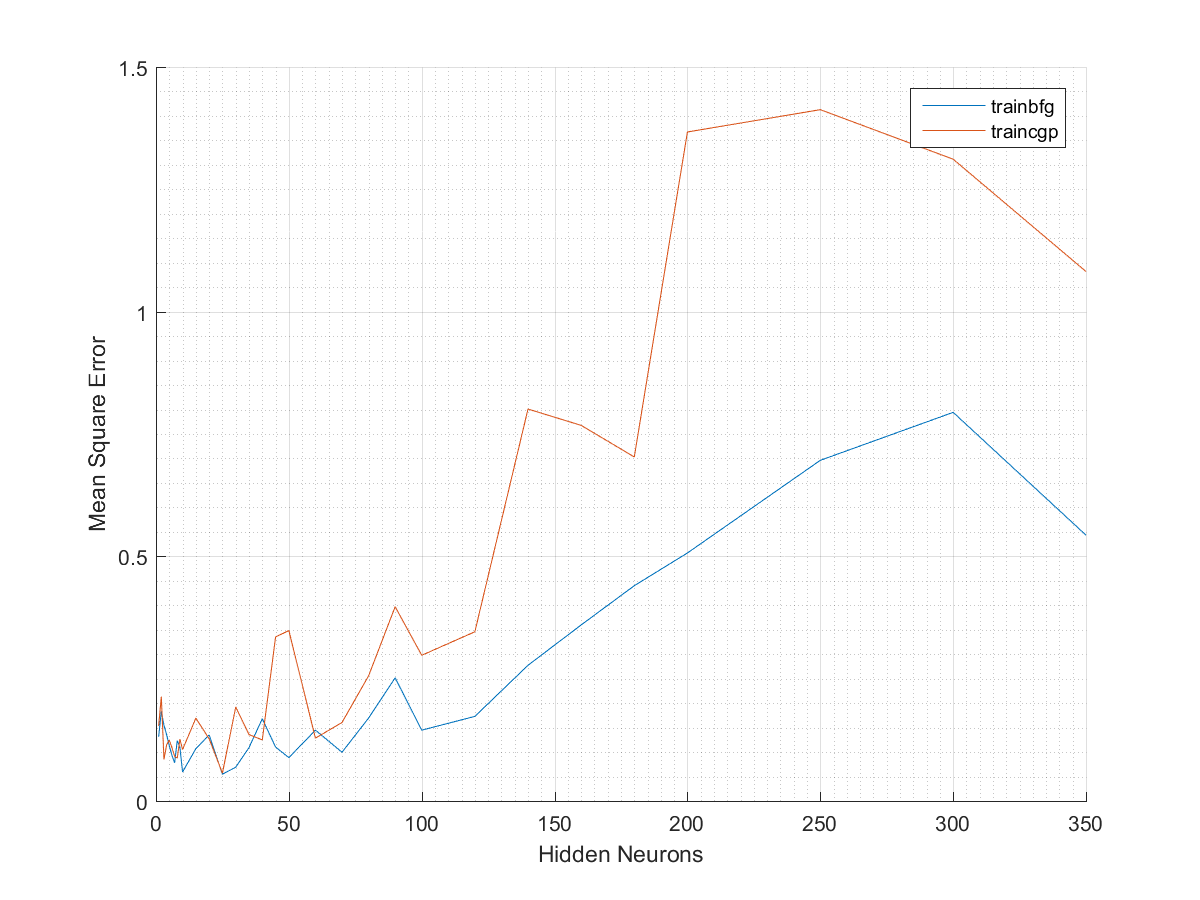
\includegraphics[width=\linewidth]{pic/unmixed_best_fullrange.png}
    \caption{MSE of best performing algorithms}
    \label{fig:unmixed_full}
\end{figure}

\begin{figure}[!ht]
    \centering
    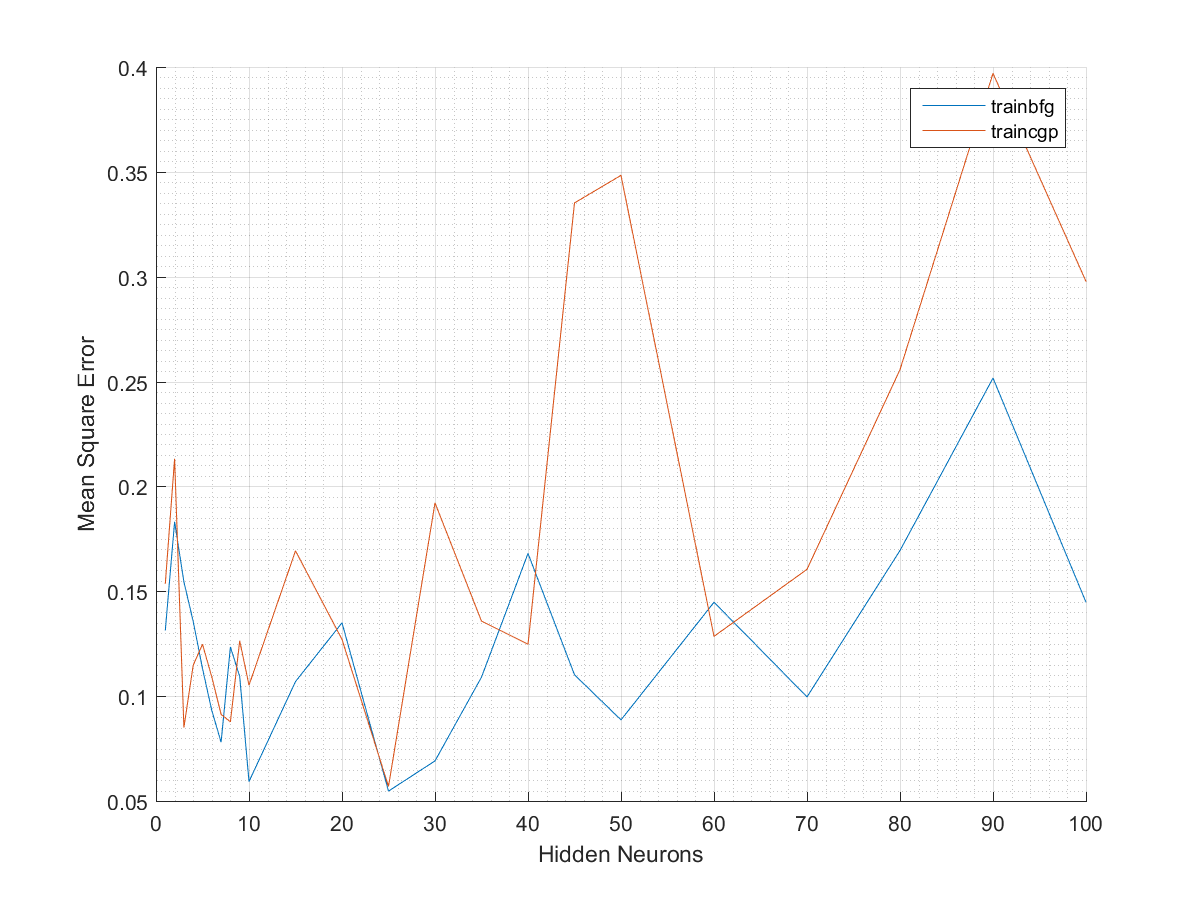
\includegraphics[width=\linewidth]{pic/unmixed_best_limited.png}
    \caption{MSE of best performing algorithms with limited axis}
    \label{fig:unmixed_limited}
\end{figure}

% Should I add a bar chart or something of all training algorithms with their MMSE between 1-100 neurons?

% TODO some discussion of the results. Why is it darting up and down so much? Can you see a down-curve of underfitting, then an up-curve of overfitting? What's the OPTIMAL number of neurons to use? (25) What's the best algorithm overall? Why?

% TODO show a table of data around the point of interest, 25 neurons. 10-40 for each, perhaps? trainbfh, traincgp

\begin{table}
\centering
\caption{Raw data of best performing algorithms}
\label{tbl:unmixed}
\begin{tabular}{llllll}
\hline
\textbf{Algorithm} & \textbf{Neurons} & \textbf{Time to Train (s)} & \textbf{Accuracy} & \textbf{MSE} \\ \hline
trainbfg & 15 & 0.15658 & 0.9 & 0.10695 \\ \hline 
trainbfg & 20 & 0.23614 & 0.8 & 0.13496 \\ \hline 
trainbfg & 25 & 0.82571 & 0.95 & 0.054725 \\ \hline 
trainbfg & 30 & 0.76897 & 0.95 & 0.069127 \\ \hline 
trainbfg & 35 & 0.70948 & 0.85 & 0.10906 \\ \hline

traincgp & 15 & 0.066146 & 0.825 & 0.16928 \\ \hline 
traincgp & 20 & 0.09904 & 0.875 & 0.12706 \\ \hline 
traincgp & 25 & 0.10311 & 0.95 & 0.05694 \\ \hline 
traincgp & 30 & 0.075015 & 0.85 & 0.19212 \\ \hline 
traincgp & 35 & 0.11164 & 0.85 & 0.13576 \\ \hline 
\end{tabular}
\end{table}

The experiment was then repeated after randomly shuffling the data and partitioning again. The results for this changes on every test set due to the random element. The results are shown in Figures \ref{fig:mixed_full} and \ref{fig:mixed_limited}, as with the standard partition data.

\begin{figure}[!ht]
    \centering
    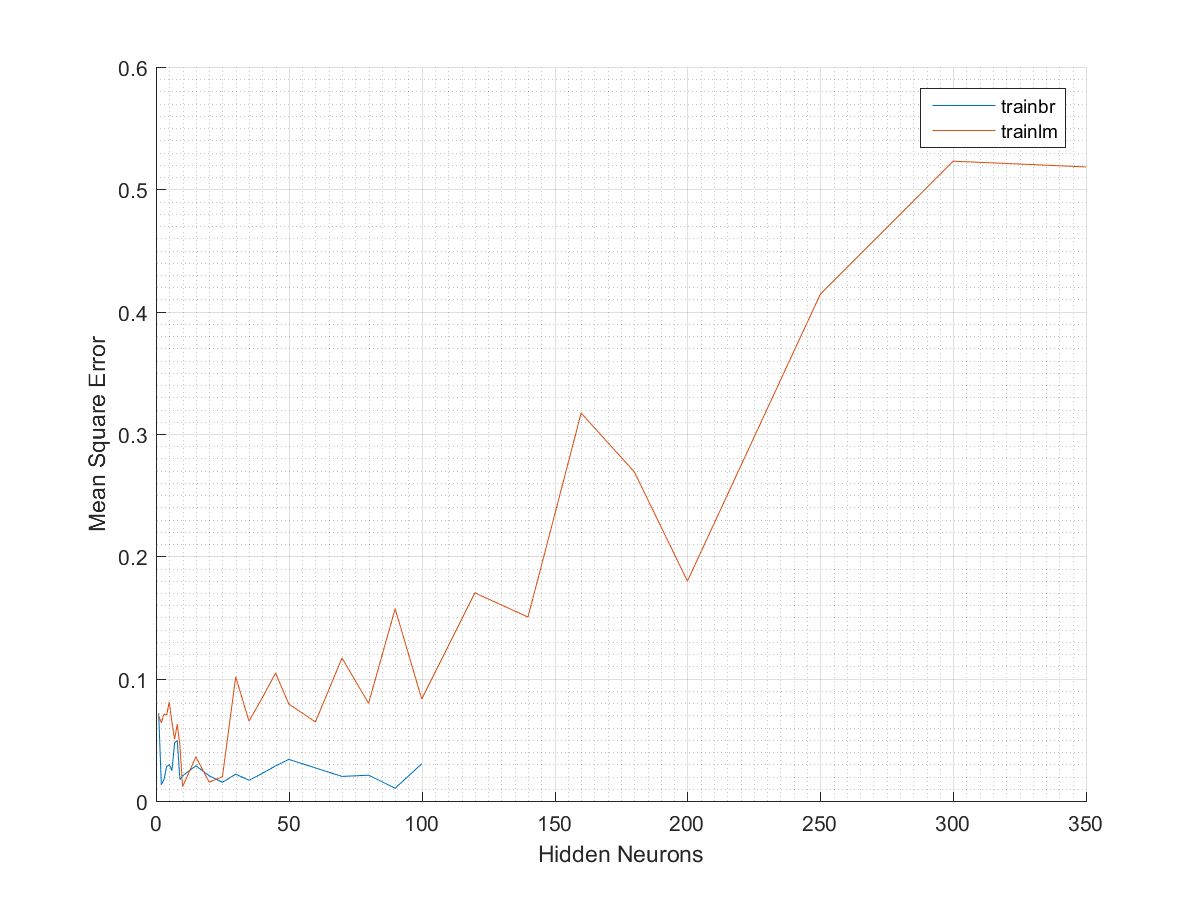
\includegraphics[width=\linewidth]{pic/mixed_best_fullrange.png}
    \caption{MSE of best performing algorithms with random partition}
    \label{fig:mixed_full}
\end{figure}

\begin{figure}[!ht]
    \centering
    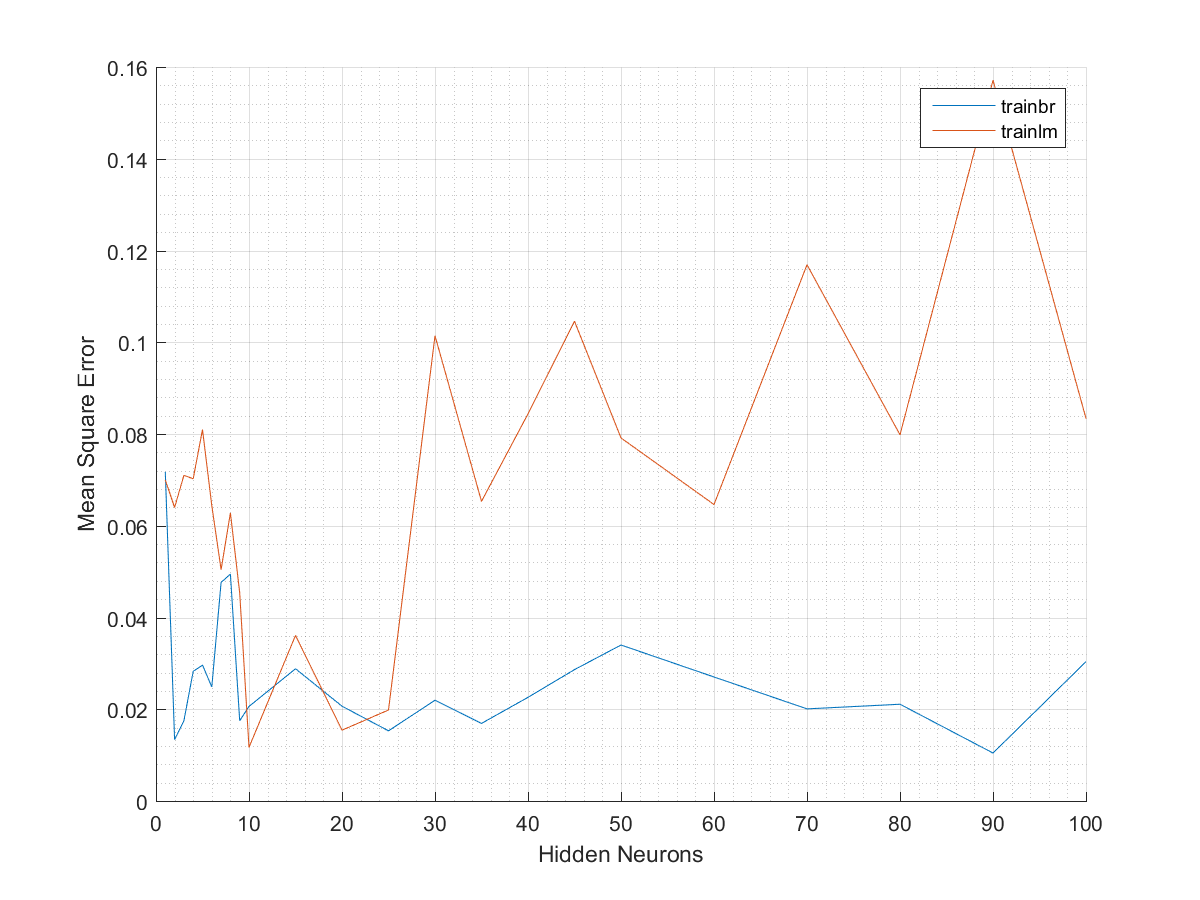
\includegraphics[width=\linewidth]{pic/mixed_best_limited.png}
    \caption{MSE of best performing algorithms with limited axis with random partition}
    \label{fig:mixed_limited}
\end{figure}

\begin{table}
\centering
\caption{Raw data of best performing algorithms in random partition}
\label{tbl:mixed}
\begin{tabular}{llllll}
\hline
\textbf{Algorithm} & \textbf{Neurons} & \textbf{Time to Train (s)} & \textbf{Accuracy} & \textbf{MSE} \\ \hline
trainbr & 15 & 5.8827 & 0.975 & 0.028823 \\ \hline 
trainbr & 20 & 8.1333 & 0.975 & 0.020667 \\ \hline 
trainbr & 25 & 14.6828 & 1 & 0.015294 \\ \hline 
trainbr & 30 & 20.2646 & 0.975 & 0.021972 \\ \hline 
trainbr & 35 & 28.5412 & 1 & 0.016915 \\ \hline 

trainlm & 15 & 0.0657085 & 0.95 & 0.036084 \\ \hline 
trainlm & 20 & 0.0607793 & 1 & 0.015435 \\ \hline 
trainlm & 25 & 0.0679456 & 1 & 0.019838 \\ \hline 
trainlm & 30 & 0.0846978 & 0.85 & 0.10142 \\ \hline 
trainlm & 35 & 0.0921787 & 0.975 & 0.065321 \\ \hline 
\end{tabular}
\end{table}

% TODO a similar discussion of results to before. Add in a comparison to unmixed; why is it different? 

% We've modified to use ALL the training algorithms and attempted to use a good range of hidden neurons
% Next is to generate some interesting graphs of training algorithm accuracies, errors etc
% Can also show how matlab does the generation, validation, and shows the performance
% Discuss the data partition, the different training algorithms, how the code is done, how all the results are taken, then discuss the results themselves

% TODO Table data needs discussing, including where the test time is

% TODO following on from discussion of 

% Compare the results to other sections

%-------------------------------------------------------------------------------
% Conclusion
%-------------------------------------------------------------------------------
\section{Conclusion}

A conclusion \cite{pca}. 

%-------------------------------------------------------------------------------
% References
%-------------------------------------------------------------------------------
\bibliographystyle{unsrt}
\bibliography{pr_refs}

%-------------------------------------------------------------------------------
% Appendix(ces)
%-------------------------------------------------------------------------------
\onecolumn
\section{Appendix} \label{sec:appendix}

\subsection*{Test set code for Task 3}
\lstinputlisting[style=Matlab-editor]{src/task3_all.m}
\newpage

\subsection*{Making and testing of neural network}
\lstinputlisting[style=Matlab-editor]{src/make_test_nn.m}
\newpage

\end{document}